\documentclass[11pt,letterpaper]{article}
\usepackage[utf8]{inputenc}
\usepackage[T1]{fontenc}
\usepackage[margin=1in]{geometry}
\usepackage{graphicx}
\usepackage{caption}
\usepackage{setspace}

\setlength{\parindent}{0pt}
\setlength{\parskip}{1em}
\pagestyle{empty}

\begin{document}

% ---------------------------------------------------------
% PAGE 1: Title and Artist Statement
% ---------------------------------------------------------
\begin{center}
    {\Huge \textbf{Assignment 4: Final Project}} \\[3em]
    
    {\large \textit{Havi Arji}} \\[5em]
\end{center}

\vspace{2em}

\noindent \textbf{Theme Selection:} \textit{Portrait Series / Conceptual Photography}

\vspace{1em}

\begin{doublespace}
This series looks at the emotional tension that can appear when animals are photographed in captivity. Instead of showing the zoo as a place of entertainment, I wanted to show it as a space of distance, observation, and reflection. By focusing on the animals’ faces and expressions, I tried to present them as individuals rather than just attractions. Using black and white helps unify the series and brings more attention to texture, contrast, and especially their eyes. Some animals seem to look directly at the viewer, while others seem tired, distant, or partly hidden, which adds to the feeling of separation. Overall, these photos are meant to feel more personal and emotional, encouraging the viewer to think about captivity, presence, and the way we look at animals.
\end{doublespace}

\newpage

% ---------------------------------------------------------
% PAGE 2: Image 1
% ---------------------------------------------------------
\vspace*{\fill}
\begin{center}
    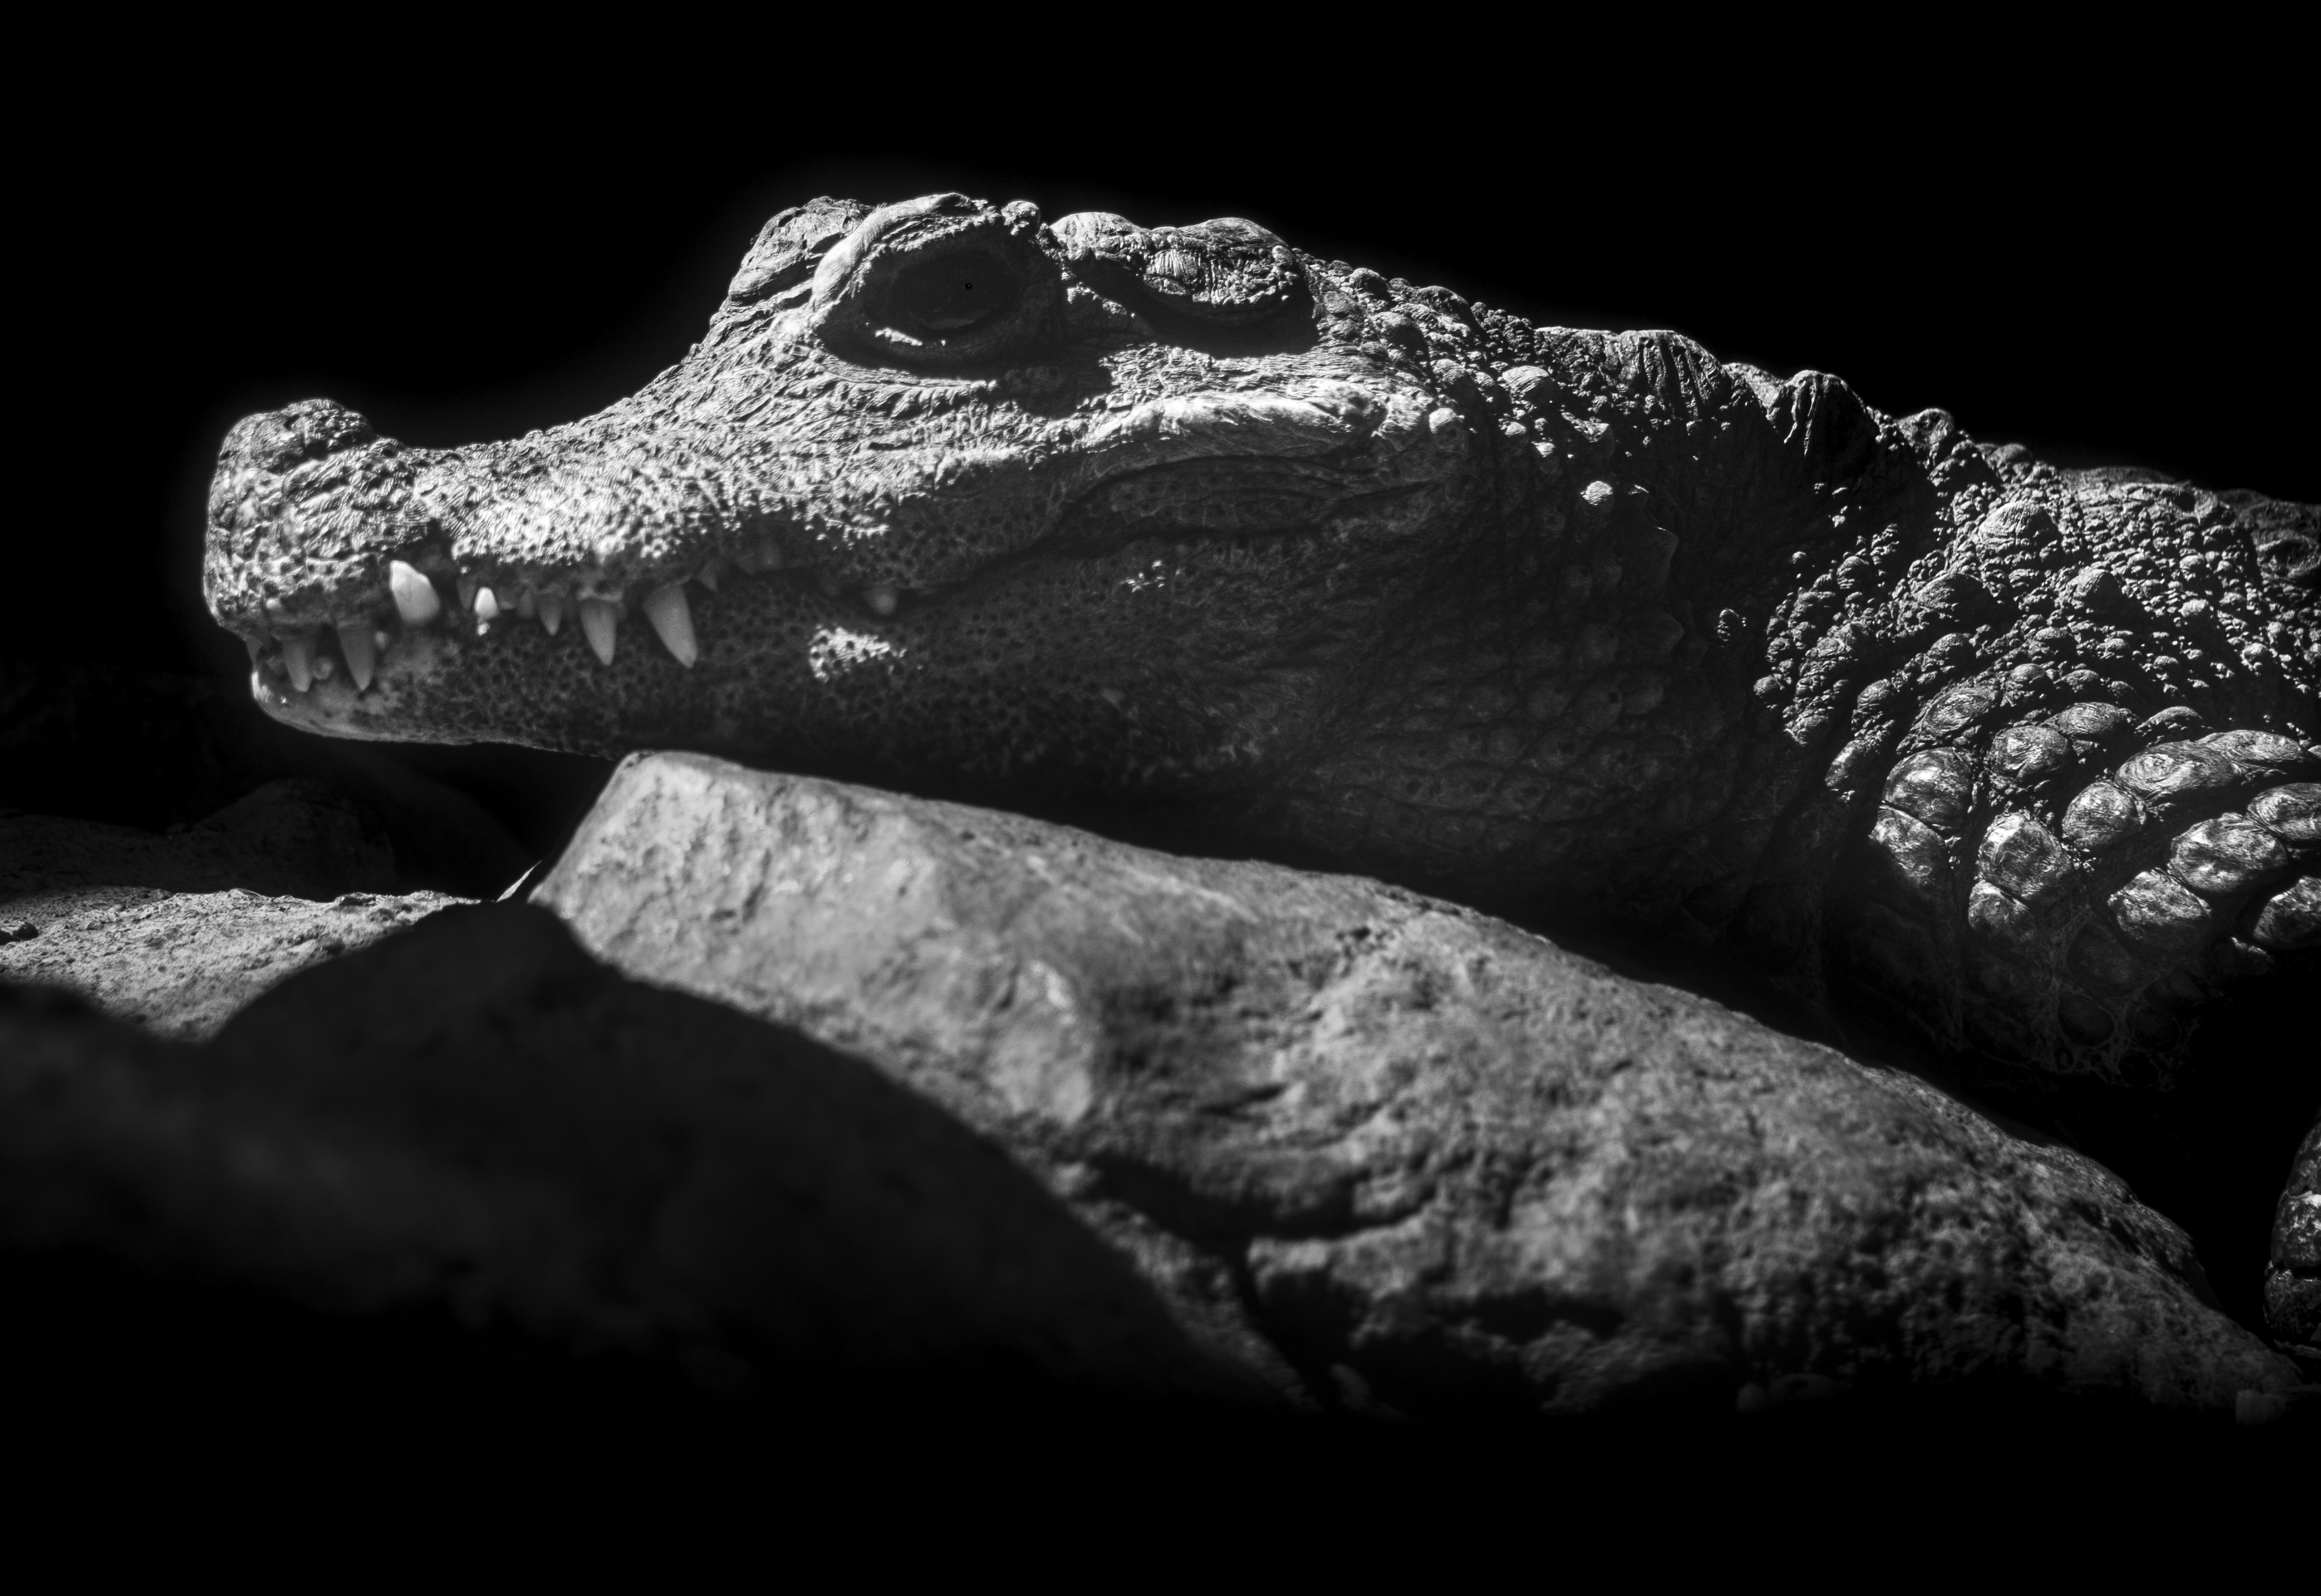
\includegraphics[width=\textwidth,height=0.7\textheight,keepaspectratio]{DSC04567.png}

    \vspace{1.5em}
    {\Large \textbf{Stillness in the Dark}} \\[0.8em]
    \textbf{Camera:} Sony NEX-5R \\
    \textbf{Aperture:} f/4.5 \quad \textbf{ISO:} 200 \quad \textbf{Shutter Speed:} 1/160s \quad \textbf{Focal length:} 70mm \\[0.5em]
    \textit{A close portrait of a crocodile emerging from shadow. The sharp texture of the scales and the heavy darkness around the body create a sense of tension, stillness, and contained power.}
\end{center}
\vspace*{\fill}
\newpage

% ---------------------------------------------------------
% PAGE 3: Image 2
% ---------------------------------------------------------
\vspace*{\fill}
\begin{center}
    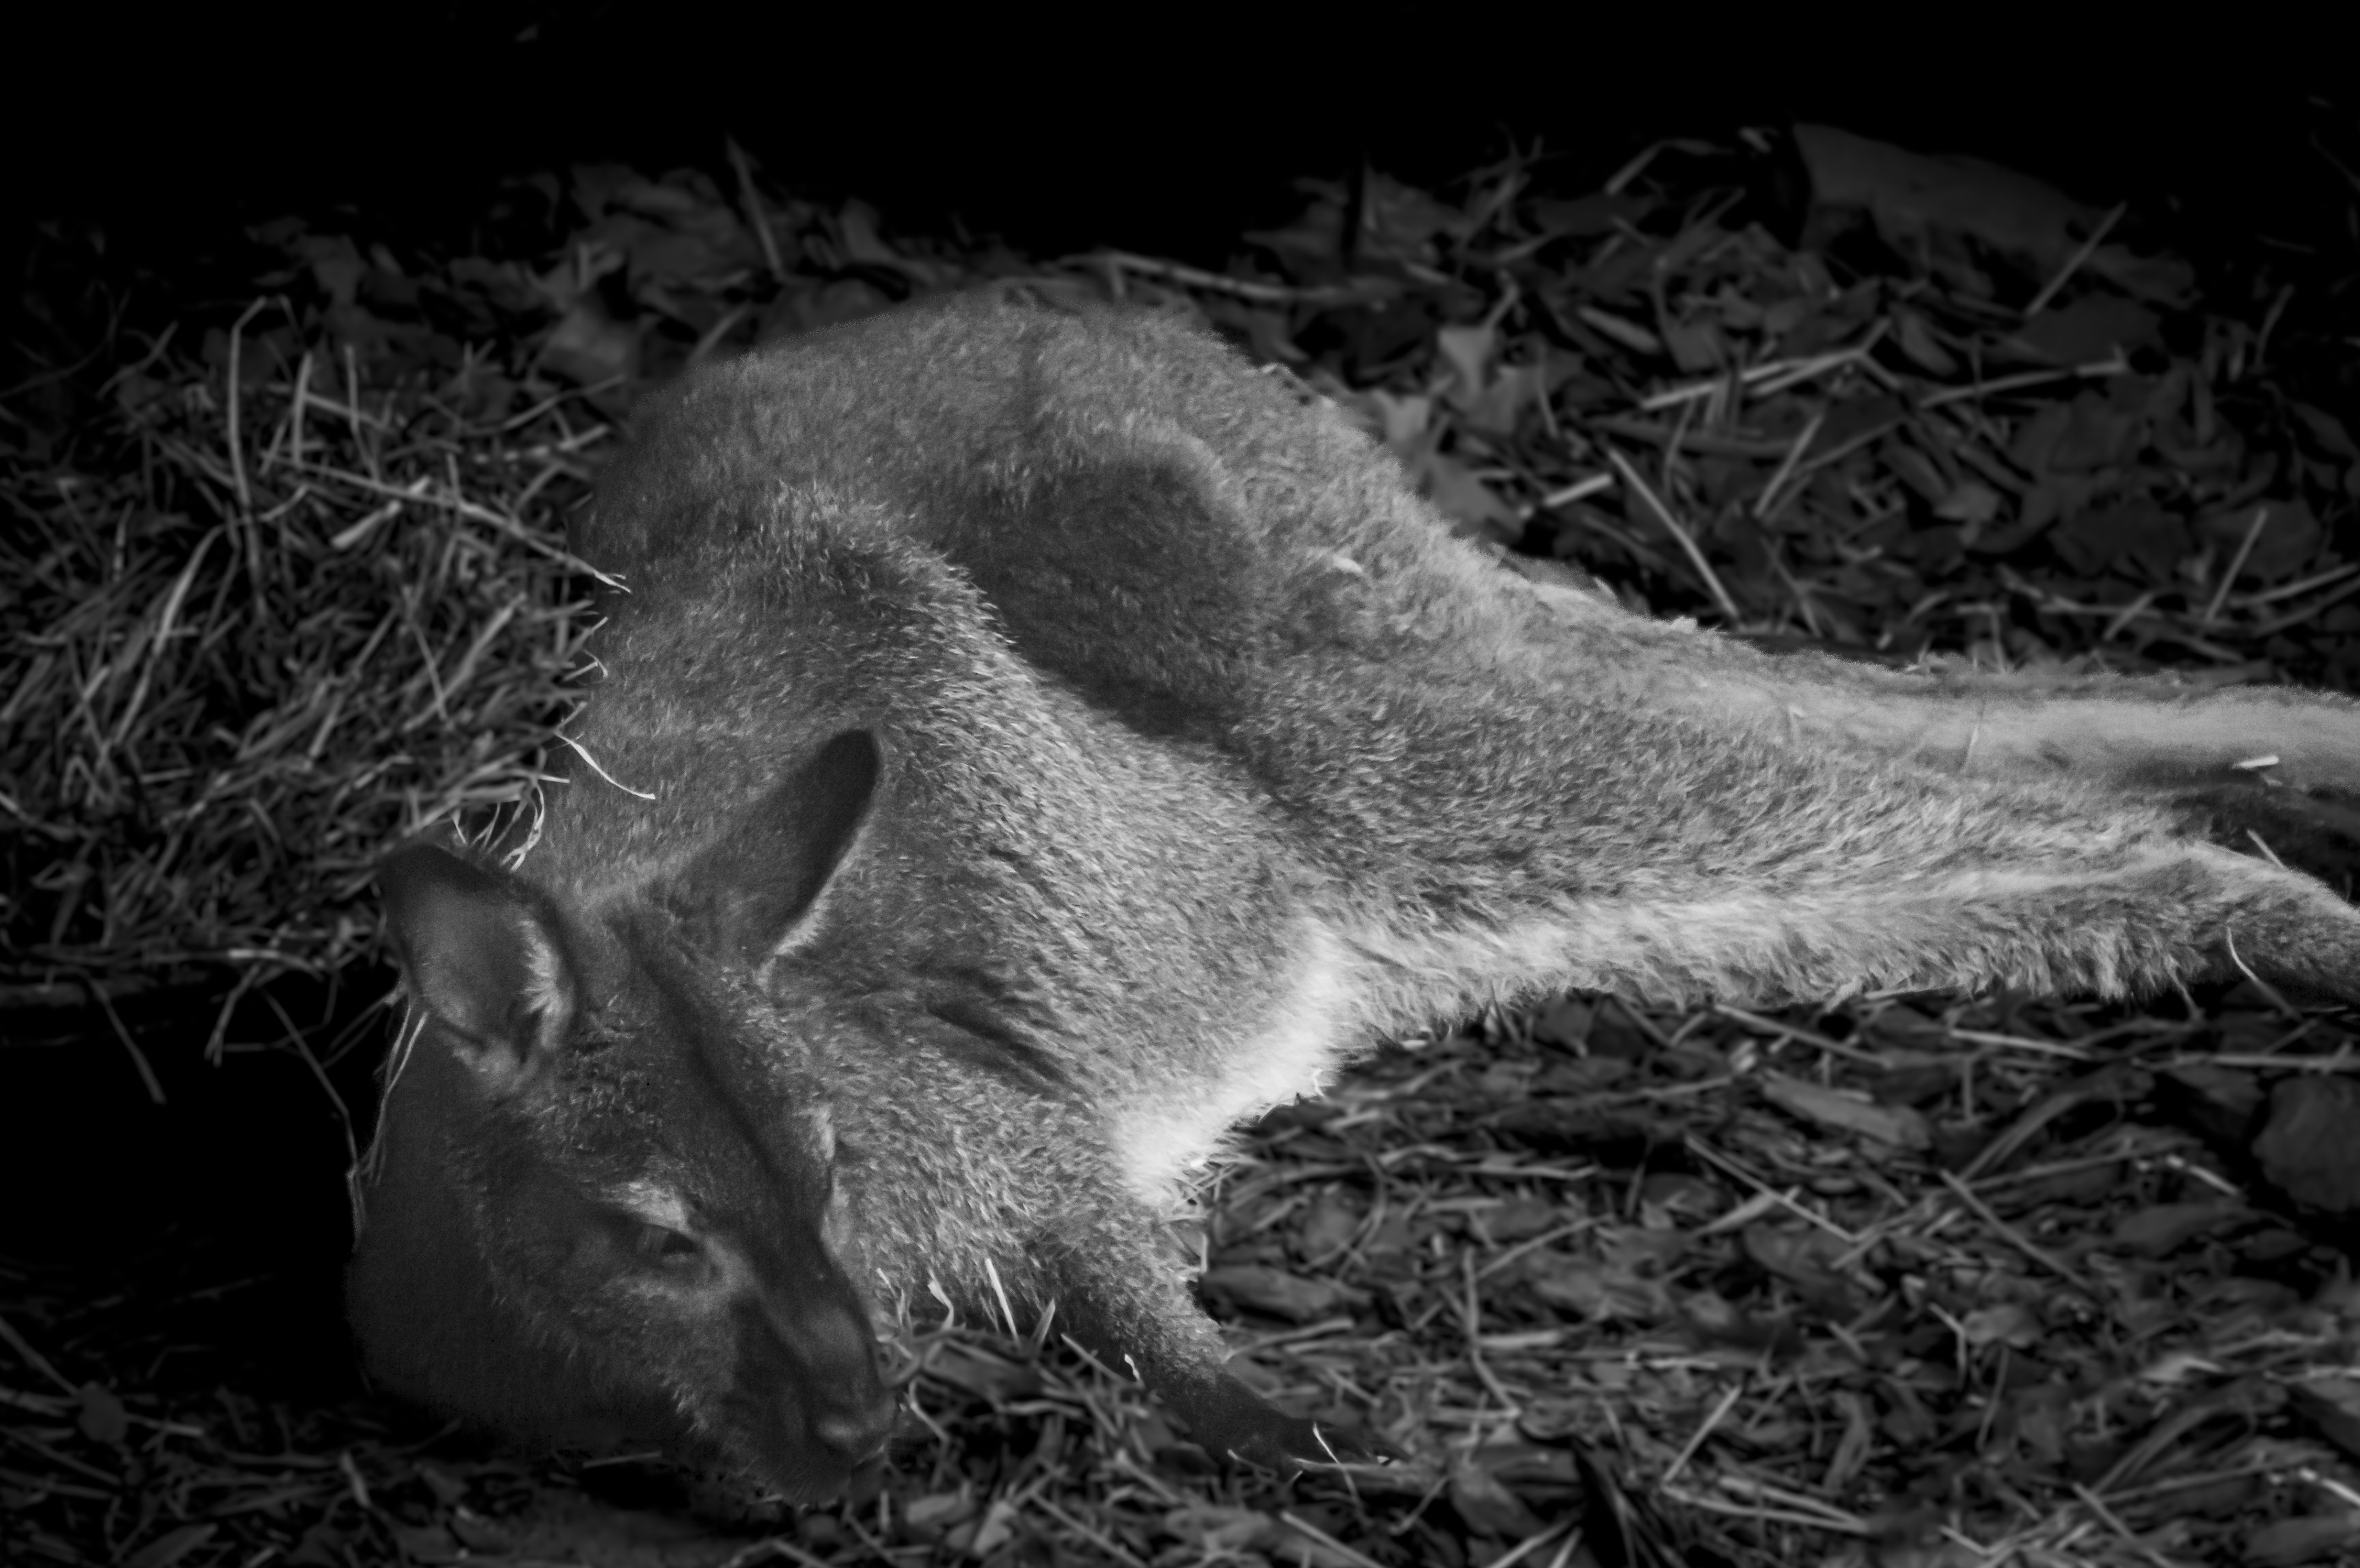
\includegraphics[width=\textwidth,height=0.7\textheight,keepaspectratio]{DSC04579.png}

    \vspace{1.5em}
    {\Large \textbf{Resting Body}} \\[0.8em]
    \textbf{Camera:} Sony NEX-5R \\
    \textbf{Aperture:} f/6.3 \quad \textbf{ISO:} 300 \quad \textbf{Shutter Speed:} 1/50s \quad \textbf{Focal length:} 210mm \\[0.5em]
    \textit{This image shows a kangaroo-like animal lying low against the ground. Its posture suggests fatigue or withdrawal, and the monochrome treatment emphasizes the quiet heaviness of the moment.}
\end{center}
\vspace*{\fill}
\newpage

% ---------------------------------------------------------
% PAGE 4: Image 3
% ---------------------------------------------------------
\vspace*{\fill}
\begin{center}
    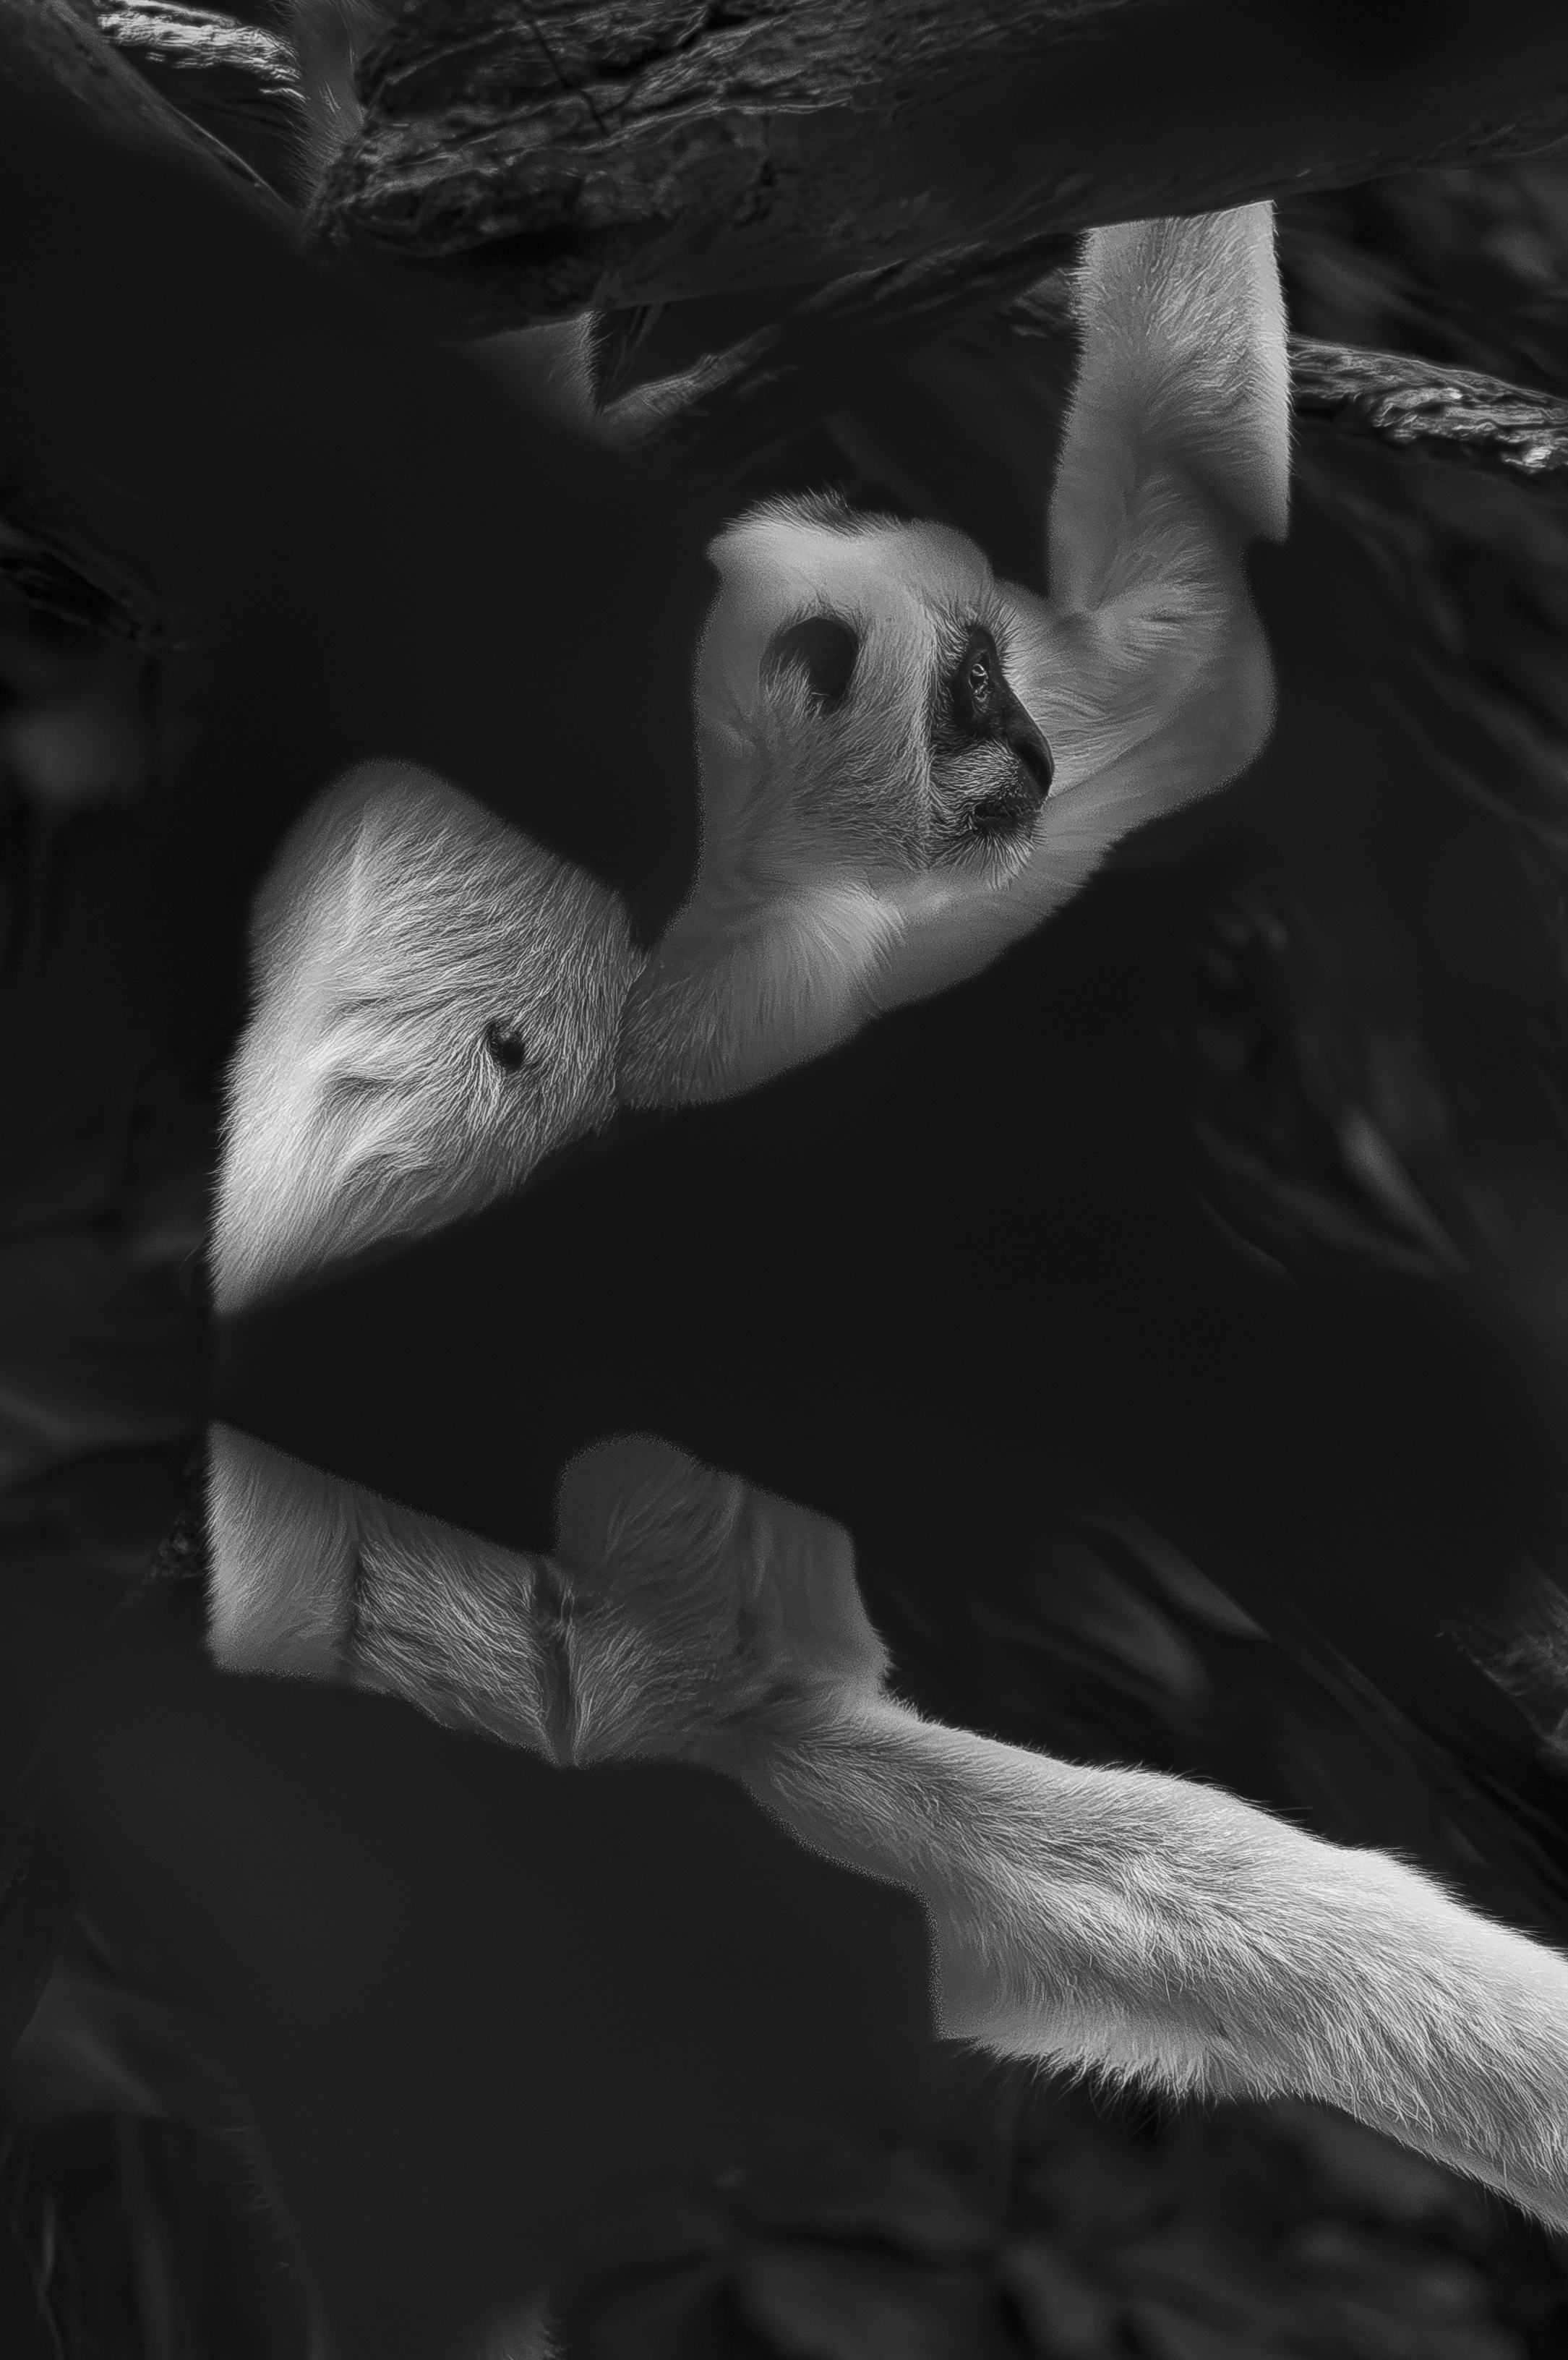
\includegraphics[width=\textwidth,height=0.7\textheight,keepaspectratio]{DSC04586.png}

    \vspace{1.5em}
    {\Large \textbf{Obstructed View}} \\[0.8em]
    \textbf{Camera:} Sony NEX-5R \\
    \textbf{Aperture:} f/5.6 \quad \textbf{ISO:} 3200 \quad \textbf{Shutter Speed:} 1/250s \quad \textbf{Focal length:} 138mm\\[0.5em]
    \textit{Partially hidden behind branches, this primate appears both present and inaccessible. The visual barriers in the frame reinforce the theme of separation, distance, and confinement.}
\end{center}
\vspace*{\fill}
\newpage

% ---------------------------------------------------------
% PAGE 5: Image 4
% ---------------------------------------------------------
\vspace*{\fill}
\begin{center}
    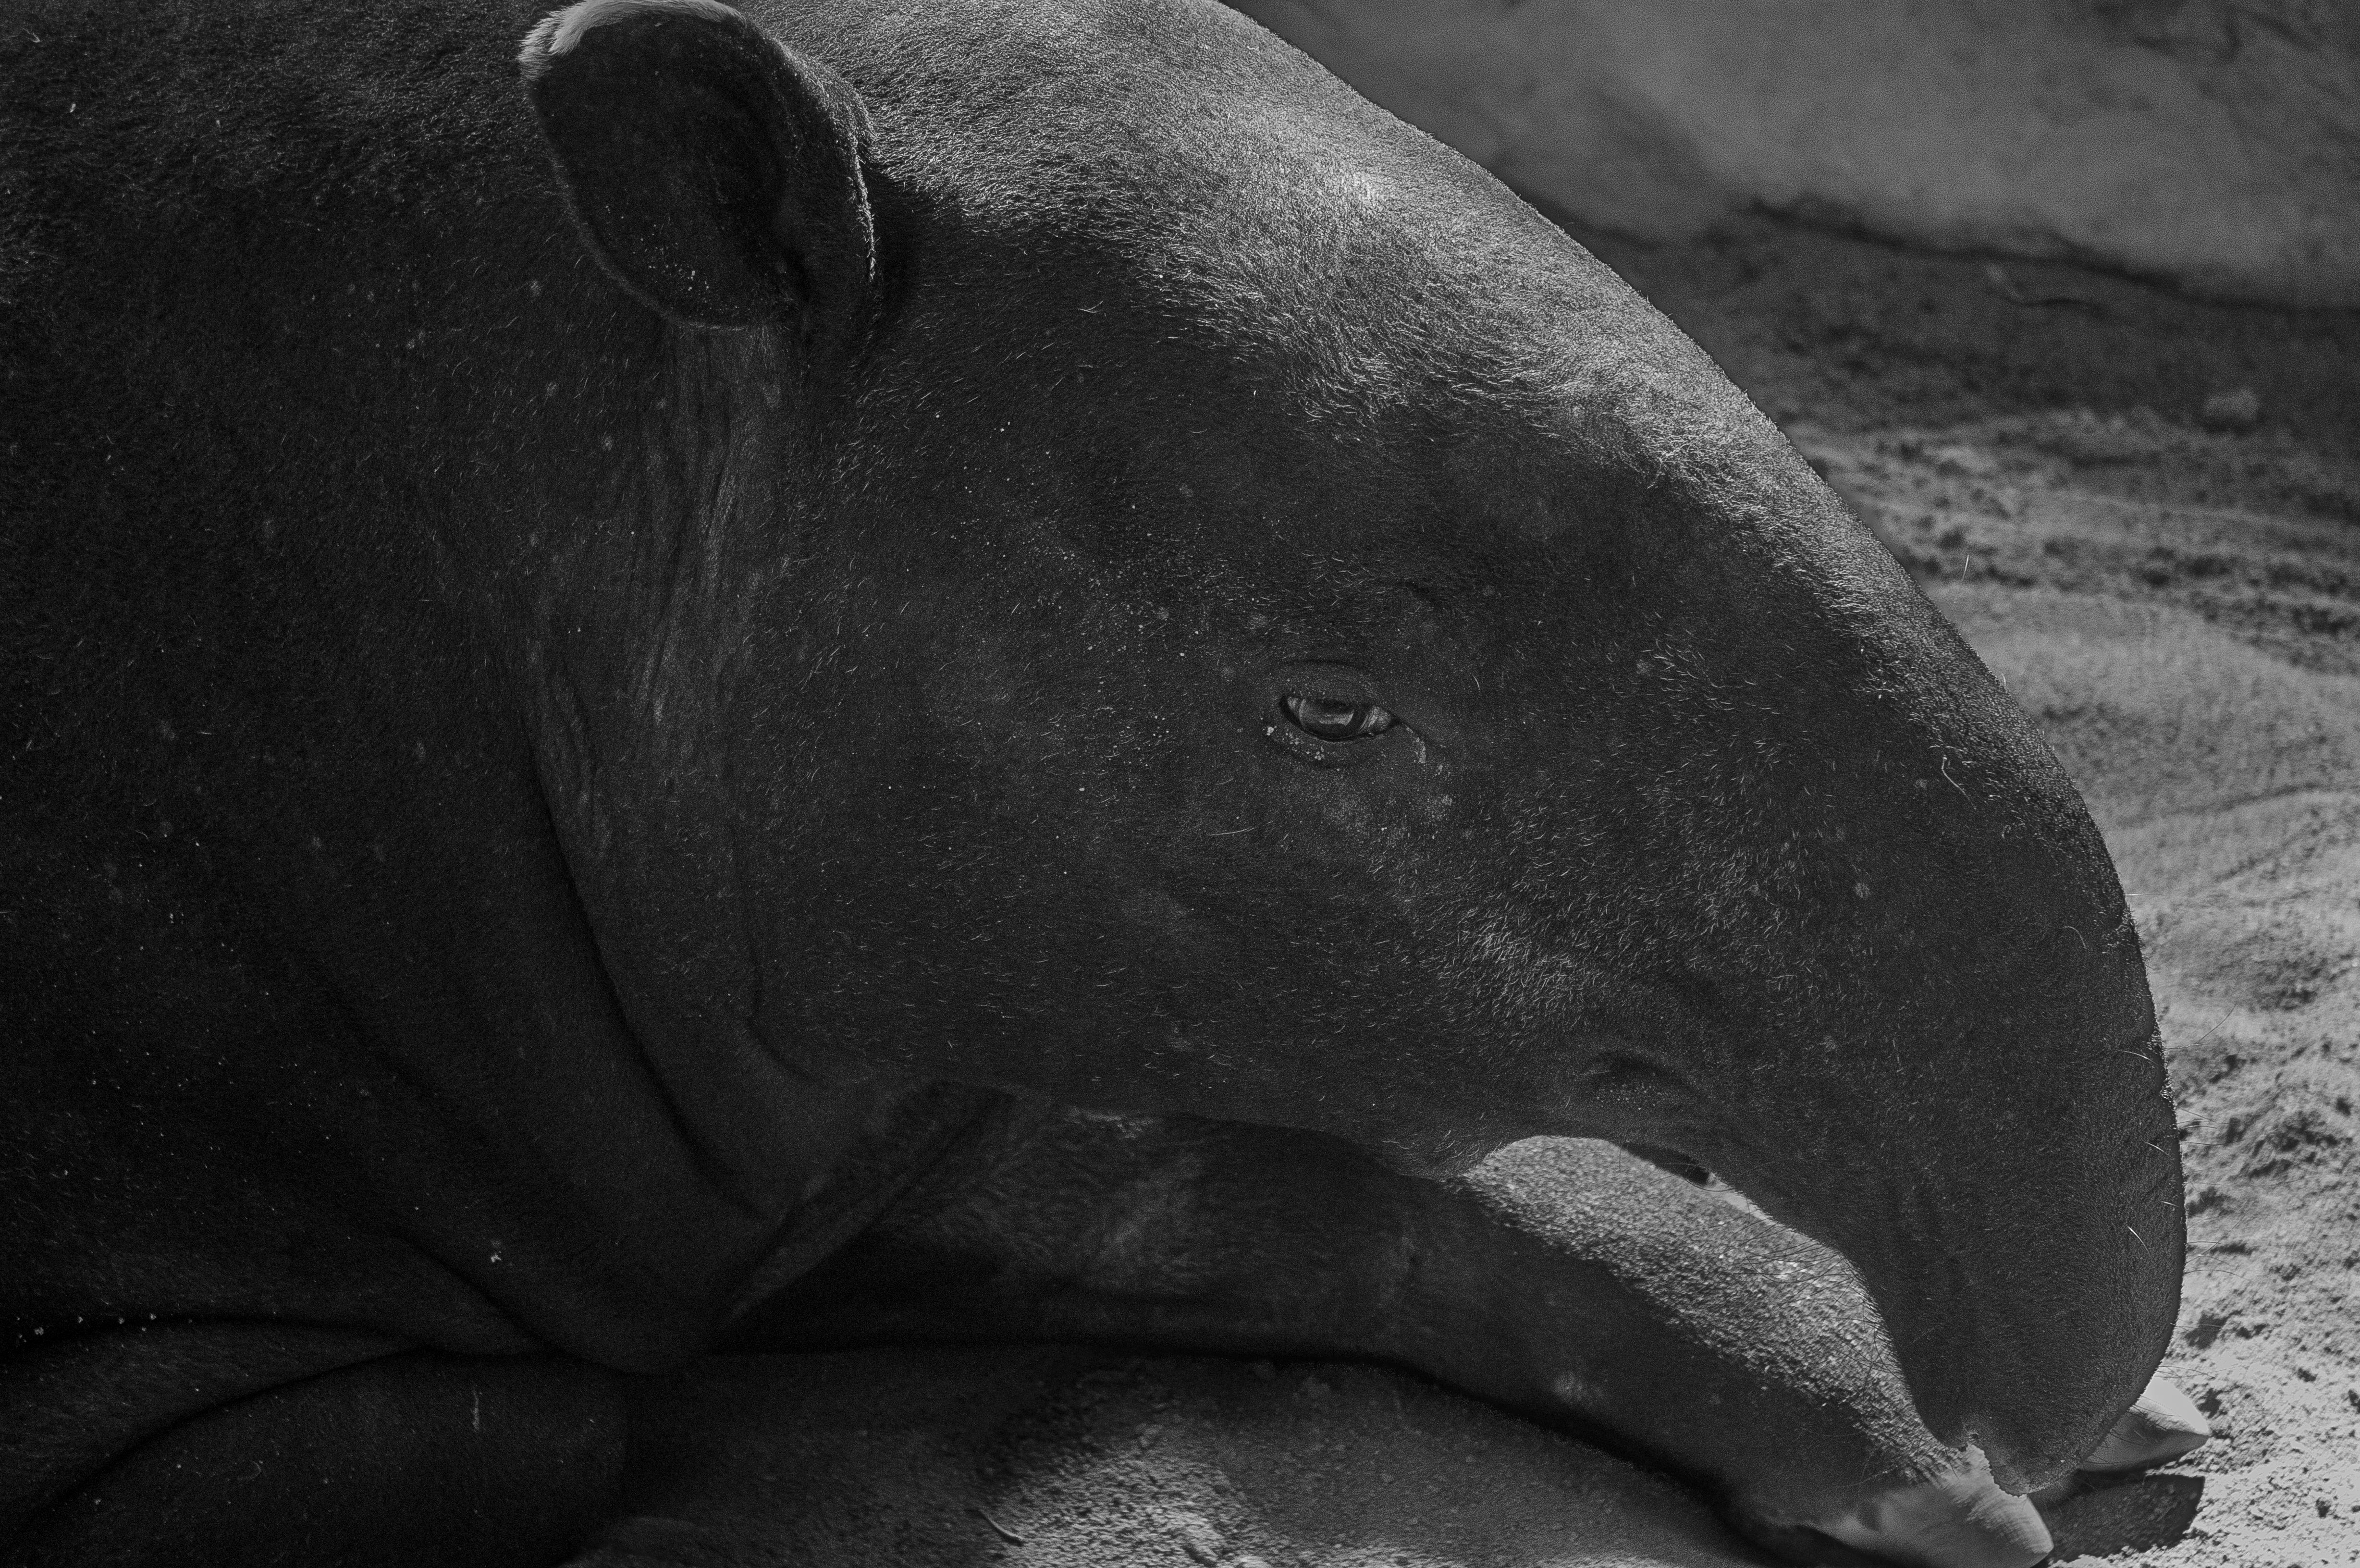
\includegraphics[width=\textwidth,height=0.7\textheight,keepaspectratio]{DSC04641-2.png}

    \vspace{1.5em}
    {\Large \textbf{Lowered Gaze}} \\[0.8em]
    \textbf{Camera:} Sony NEX-5R \\
    \textbf{Aperture:} f/5.6 \quad \textbf{ISO:}    3200 \quad \textbf{Shutter Speed:} 1/160s \quad \textbf{Focal length:} 138mm\\[0.5em]
    \textit{This close portrait of a tapir focuses on the eye and downward angle of the face. The subdued expression and soft contrast create an atmosphere of quiet sadness and introspection.}
\end{center}
\vspace*{\fill}
\newpage

% ---------------------------------------------------------
% PAGE 6: Image 5
% ---------------------------------------------------------
\vspace*{\fill}
\begin{center}
    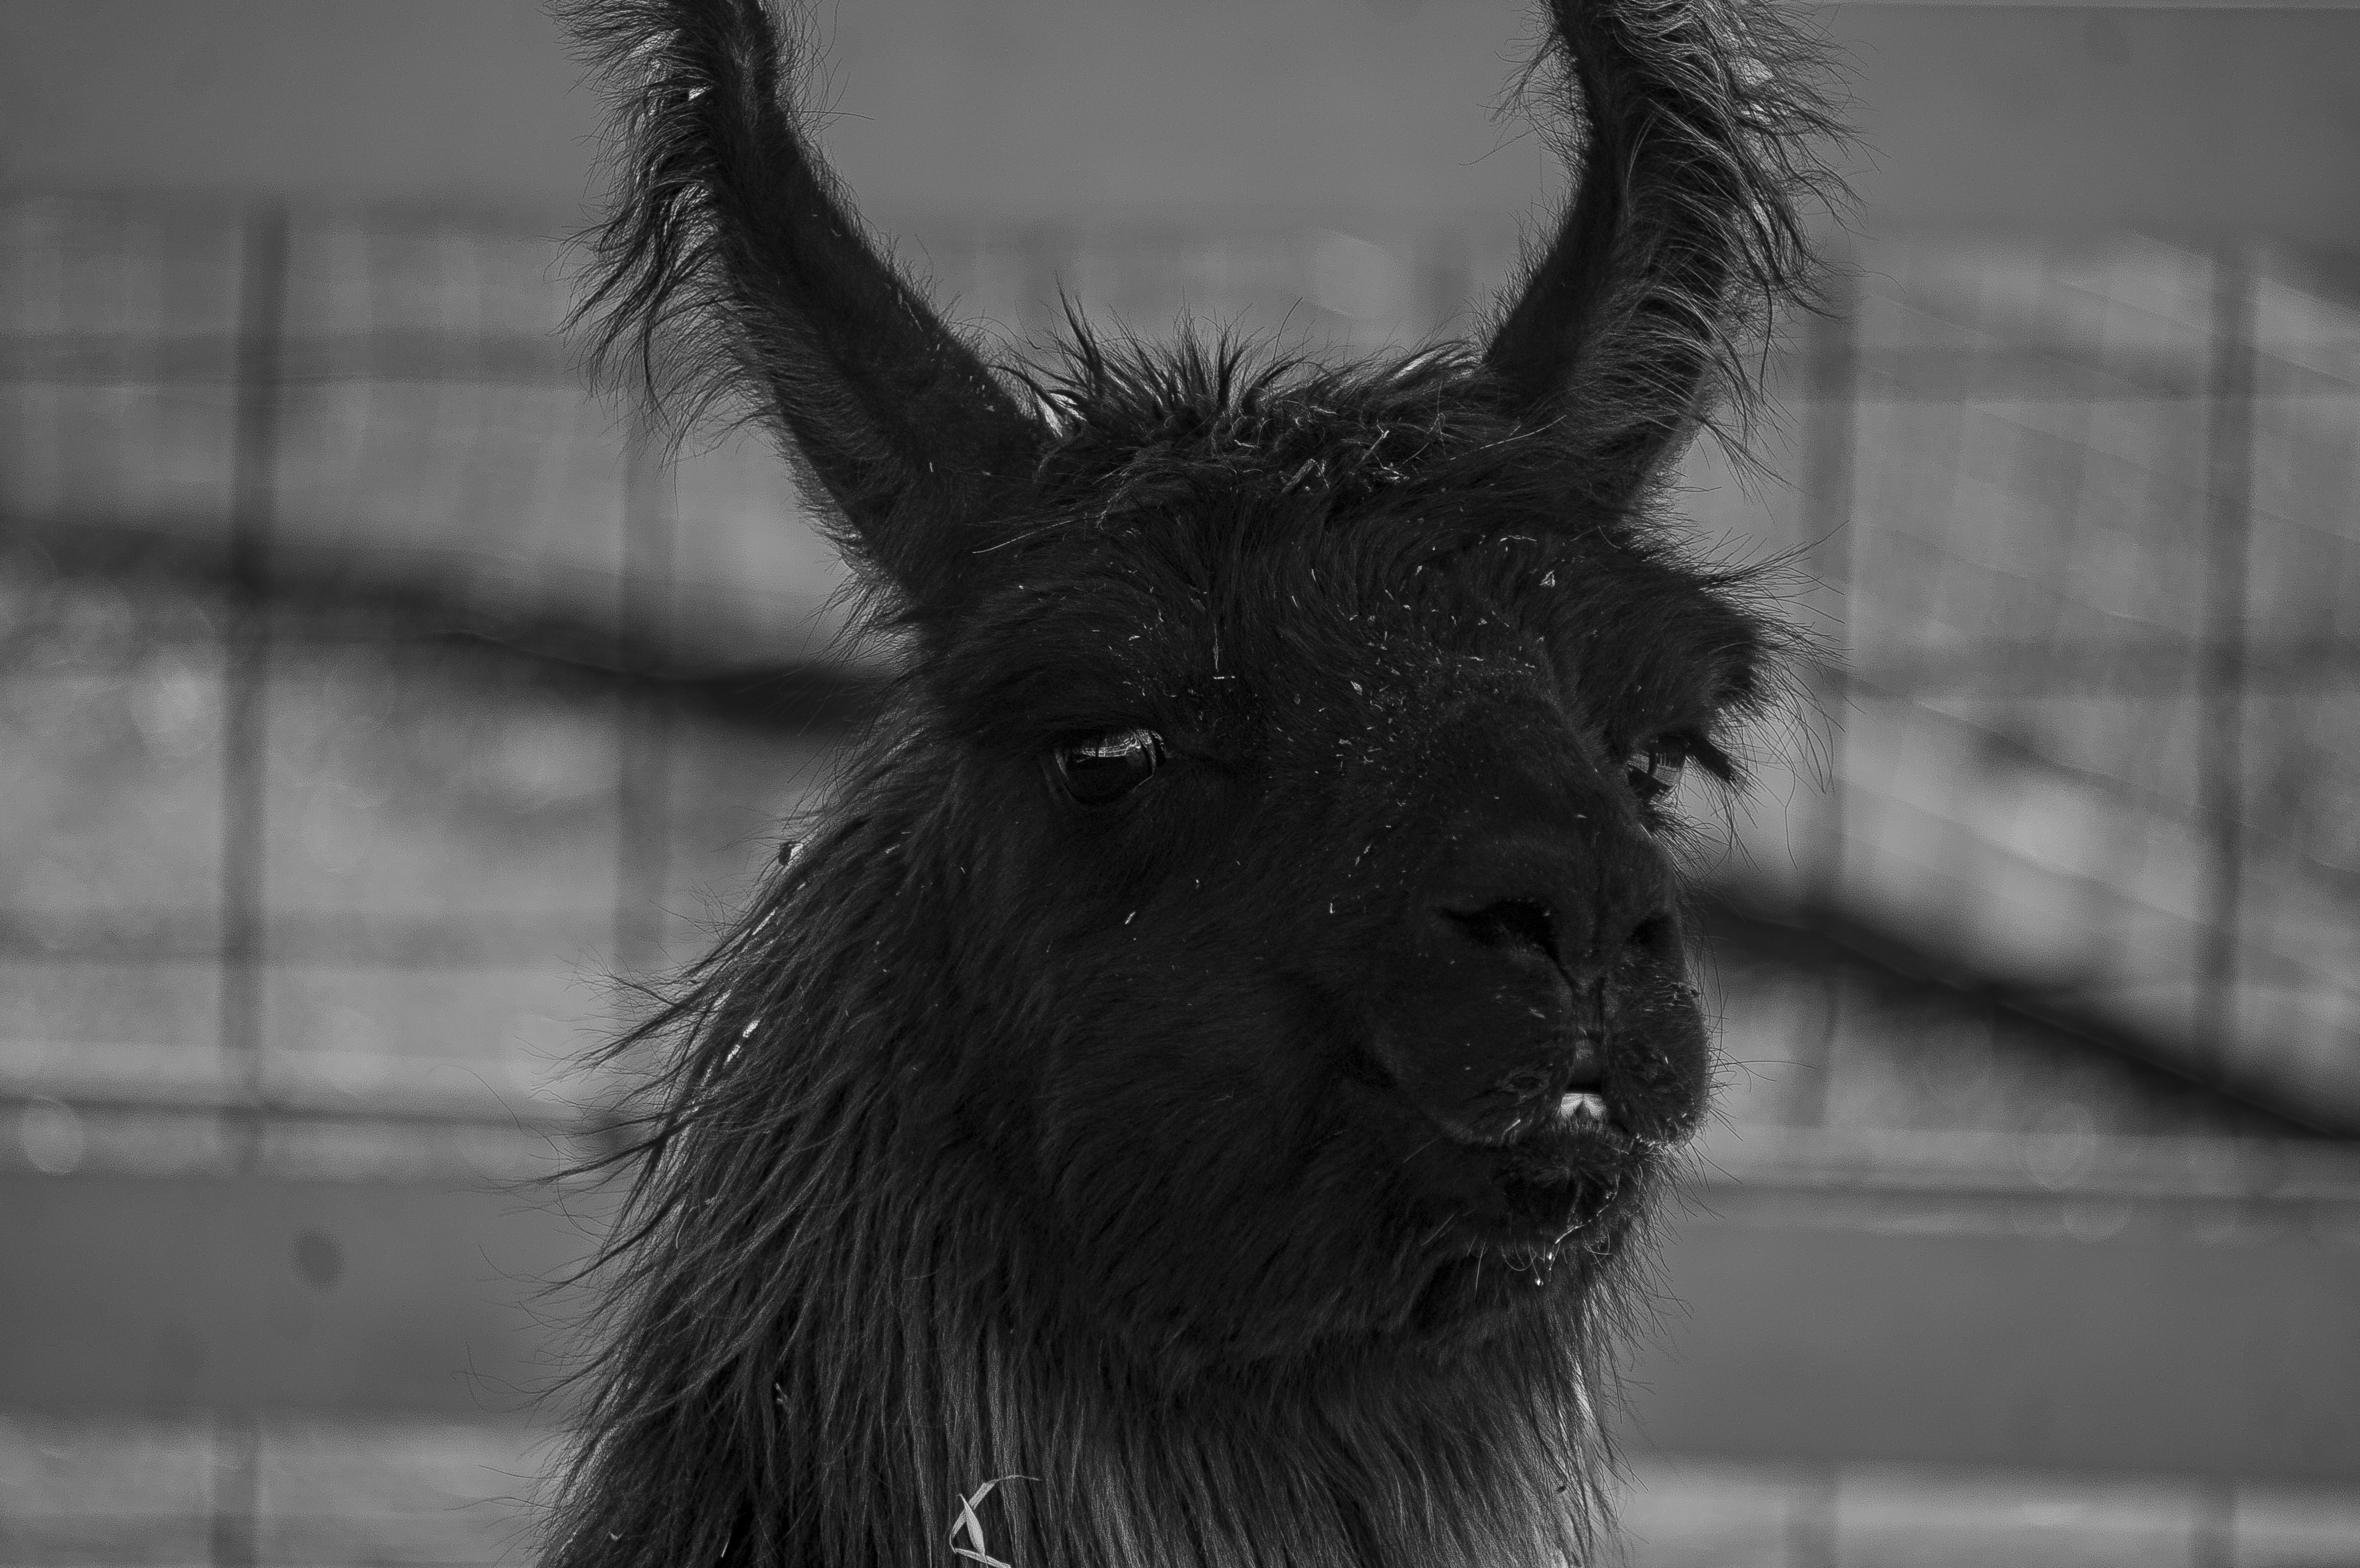
\includegraphics[width=\textwidth,height=0.7\textheight,keepaspectratio]{DSC04913.png}

    \vspace{1.5em}
    {\Large \textbf{Direct Encounter}} \\[0.8em]
    \textbf{Camera:} Sony NEX-5R \\
    \textbf{Aperture:} f/6.3 \quad \textbf{ISO:} 200 \quad \textbf{Shutter Speed:} 1/320s \quad \textbf{Focal length:} 188mm\\[0.5em]
    \textit{The llama faces the camera directly, creating an immediate sense of confrontation. Its expression is calm yet uncertain, turning the image into a portrait built around eye contact and presence.}
\end{center}
\vspace*{\fill}
\newpage

% ---------------------------------------------------------
% PAGE 7: Image 6
% ---------------------------------------------------------
\vspace*{\fill}
\begin{center}
    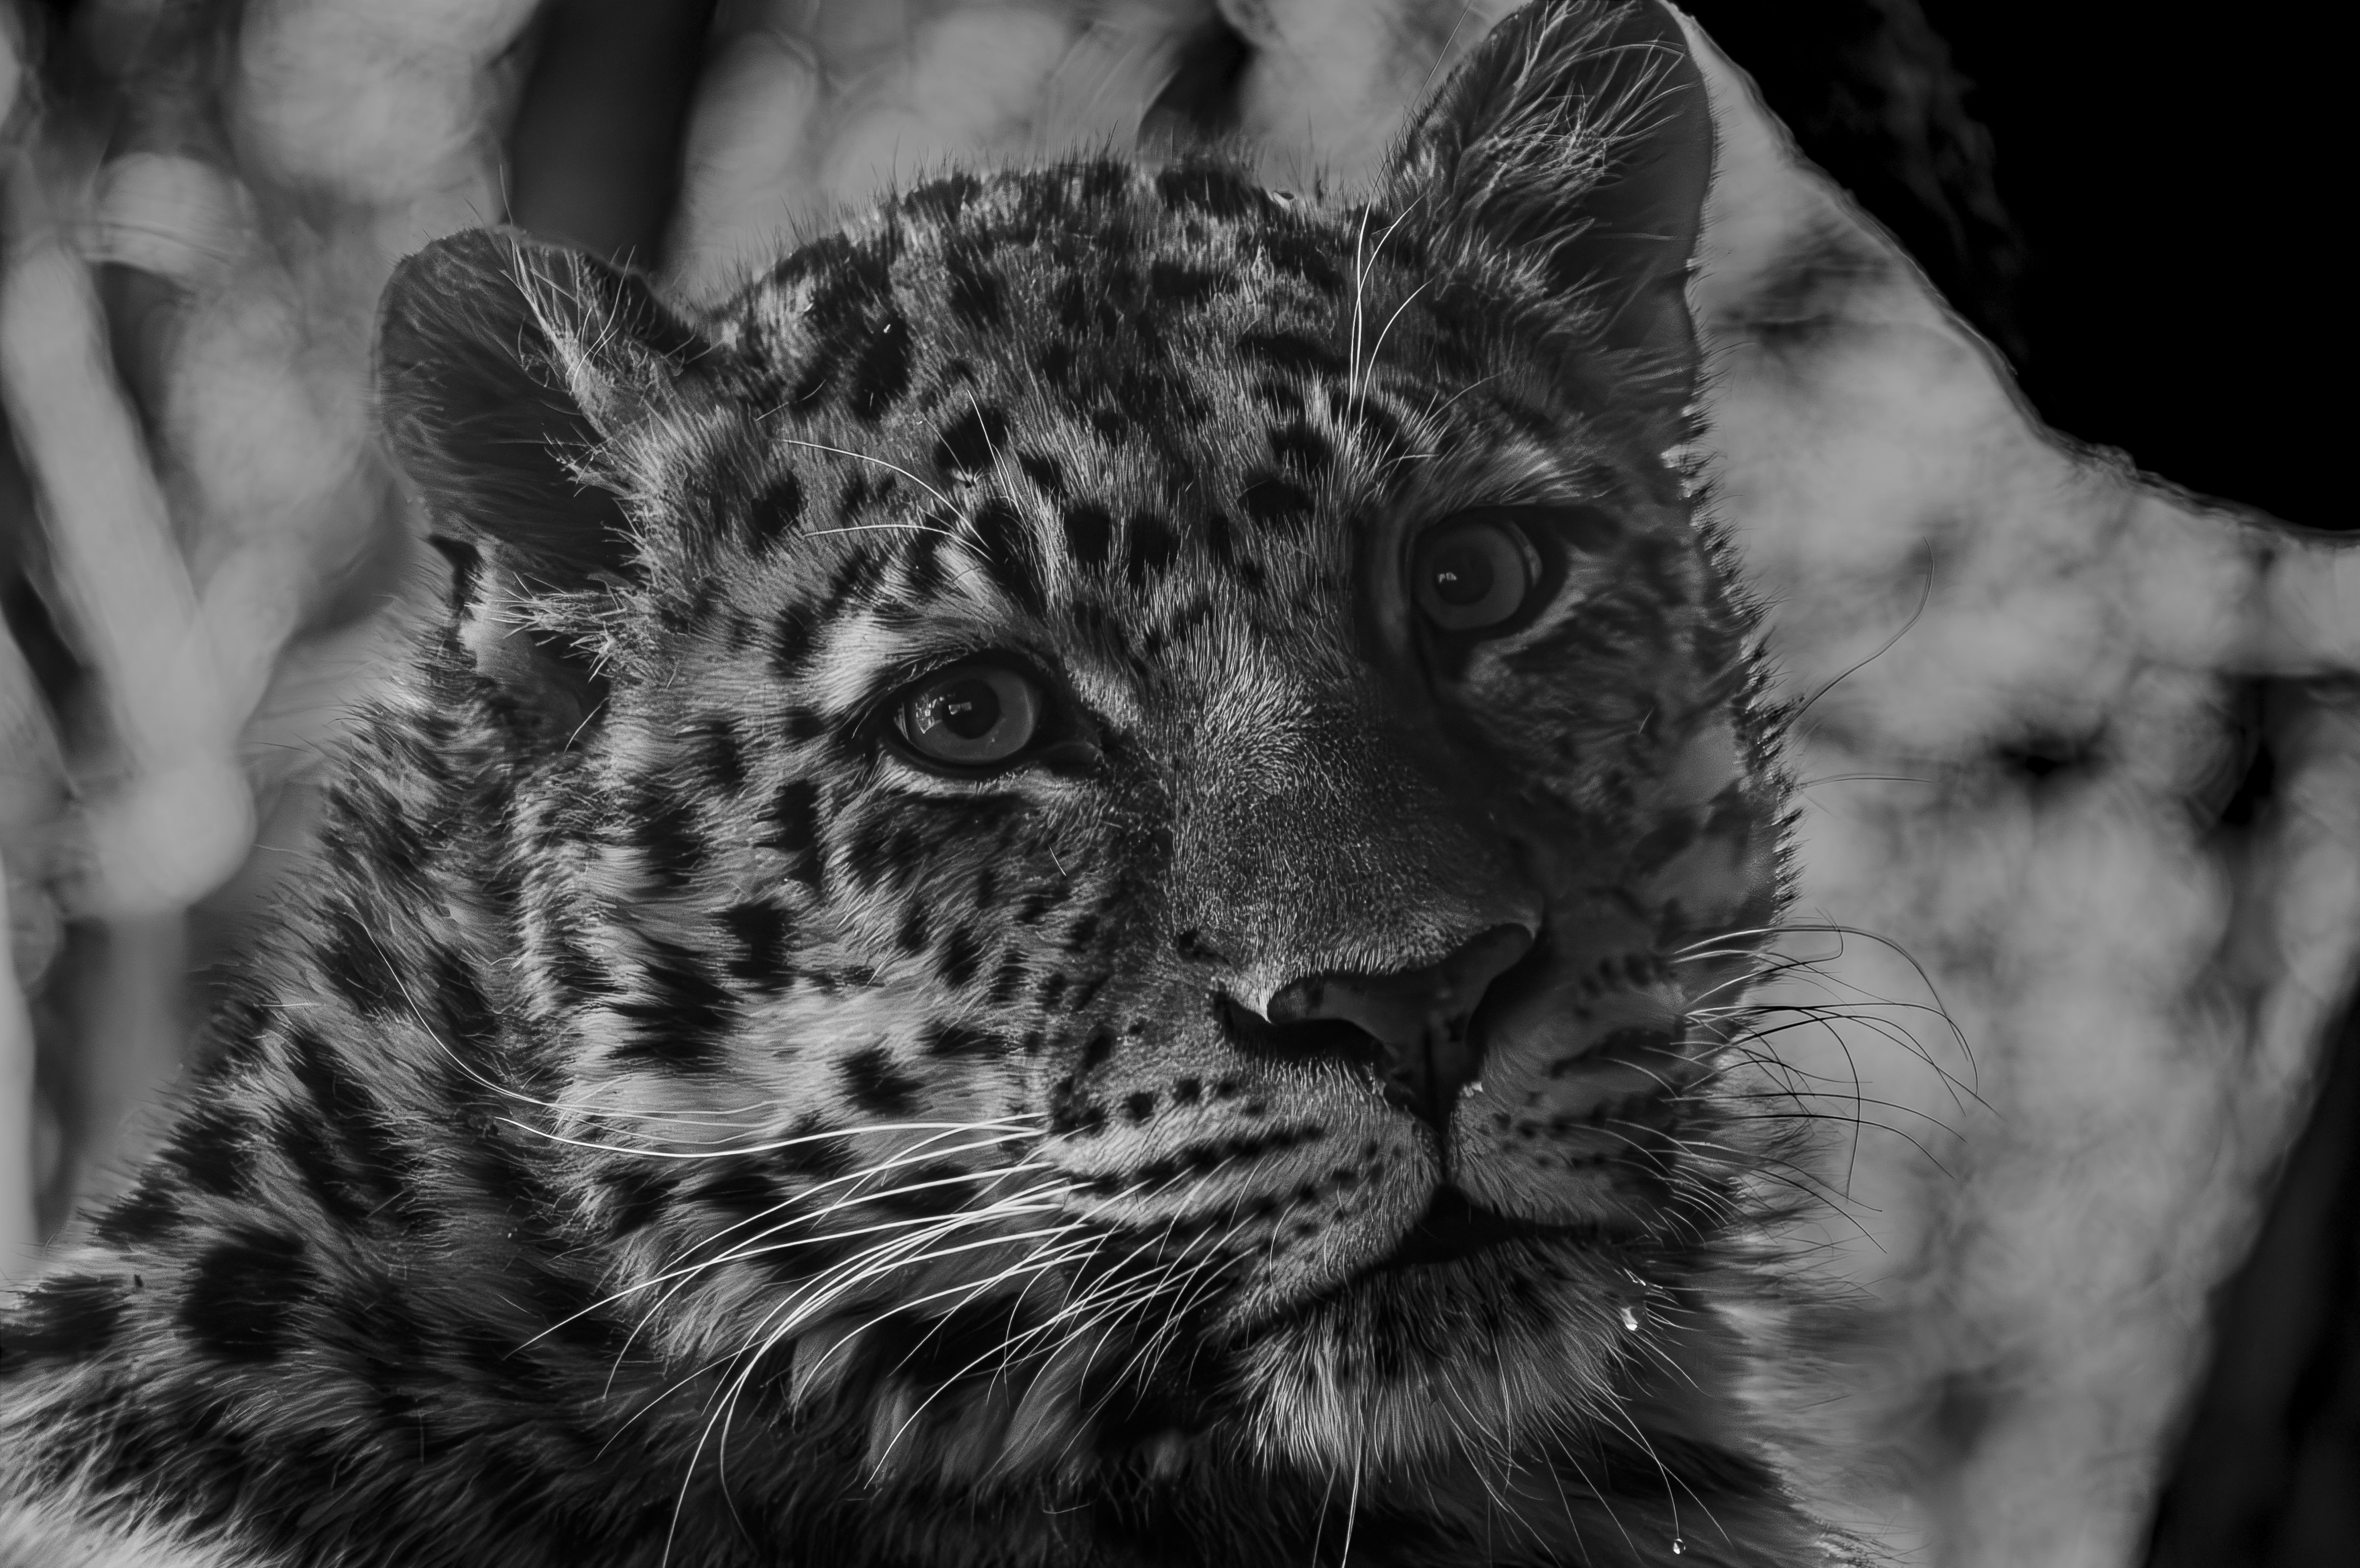
\includegraphics[width=\textwidth,height=0.7\textheight,keepaspectratio]{DSC05145.png}

    \vspace{1.5em}
    {\Large \textbf{Silent Witness}} \\[0.8em]
    \textbf{Camera:} Sony NEX-5R \\
    \textbf{Aperture:} f/6.3 \quad \textbf{ISO:} 1600 \quad \textbf{Shutter Speed:} 1/320s \quad \textbf{Focal length:} 208mm\\[0.5em]
    \textit{A direct encounter with a wild animal, showing a moment of quiet intensity and the feeling of being watched.}
\end{center}
\vspace*{\fill}

\end{document}